% =====================================================================
%  V. Results
%
%  Moi con so trong muc nay deu doc ra tu artifact trong repo va duoc
%  runners/audit_c4.py + runners/audit_figures.py doi chieu doc lap.
%  KHONG duoc go tay them so nao vao day ma khong co artifact dung sau.
%
%  Nhung cho phai giu nguyen ke ca khi doc kho chiu:
%    - XGBoost dung dau bang o C2 (0.8503 > 0.8469)
%    - SVM-RBF thang moi model ve rare-attack F1
%    - QSVM chua bao gio thang SVM-RBF co y nghia trong sweep sample size
%    - prior shift: QSVM tut nhieu hon ca hai ensemble cay
% =====================================================================

\subsection{Choosing the embedding size, and what it costs}
\label{sec:res-c1}
\revnote{rewrite}{Fig. 5 (Pareto frontier) of the submitted version removed; replaced by the K sweep and the three-stage rule on both datasets (R4-2).}
\input{figs_revision/fig_ksweep}
\begin{revbody}


The feature budget $K$ and the qubit count $n$ are not independent, and the
selection rule makes the coupling explicit.

Fig.~\ref{fig:ksweep}(a) sweeps $K$ with a classical proxy. Raw macro-$F_1$ rises
monotonically to $0.9727$ at the full $K=122$, and after projection to four
components it peaks at $0.9283$ at $K=80$; at the inherited operating point
$K=20$ the projected value is $0.9007$. So $K=20$ is not the accuracy optimum,
and we do not present it as one.

What $K=20$ is, is the largest budget the rule can serve with a four-qubit
circuit. Applying the three-stage rule of Sec.~\ref{sec:framework} at $K=20$:
the variance gate $V(n)\geq0.85$ admits $n\in\{4,\dots,10\}$; the alignment gate
$\mathrm{KTA}\geq0.95\,\mathrm{KTA}_{\max}$, with $\mathrm{KTA}_{\max}=0.2439$
at $n=5$ and hence a threshold of $0.2317$, narrows this to $\{4,5,6\}$; and
minimising $Q(n)$ selects $n^\ast=4$, that is $24$ two-qubit gates.
Fig.~\ref{fig:c1-selection} shows the three stages acting in sequence.

Re-running the same rule at larger budgets (Fig.~\ref{fig:ksweep}(b)) gives
$n^\ast = 4, 7, 8, 9$ for $K = 20, 40, 80, 122$. The mechanism is the variance
gate: spreading the same variance over more retained features pushes $V(n)$ down
at every $n$, so the gate opens later. This is the honest reading of $K=20$. It
is not an elbow in accuracy (accuracy keeps improving); it is the point at
which the circuit is still cheap. Moving from $K=20$ to $K=80$ buys $0.028$
macro-$F_1$ for the classical proxy and costs a rise from $24$ to $112$
two-qubit gates. Sec.~\ref{sec:res-width} reports what happens when that price
is actually paid.
\end{revbody}

\subsection{Does entanglement help at the operating point?}
\label{sec:res-c2}
\revnote{fix}{QSVM numbers unchanged. Adding a random forest and XGBoost (AE-4, R1-5, R2-1) changes the ordering: XGBoost 0.8503 above QSVM-ZZ 0.8469. The submitted version placed QSVM first.}
\input{figs_revision/fig_ablation}
\input{figs_revision/fig_perrun}
\begin{revbody}


At $n^\ast=4$ we compare \QSVM{} against an otherwise identical circuit with the
entangling layer removed, and against five classical baselines
(Fig.~\ref{fig:perrun}). The answer splits by what is measured.

In kernel geometry the entangling layer matters, and by a wide margin: the
paired alignment gain is $\Delta\mathrm{KTA} = +0.1378$
$[+0.1267,+0.1489]$, $d_z=8.91$. In end-task accuracy it does not resolve:
$\Delta\Fmac = +0.0114$ $[-0.0054,+0.0281]$, $p=0.23$. The interval crosses zero
and we report the comparison as inconclusive. Alignment is a property of the
Gram matrix; whether it converts into accuracy depends on the classifier and the
task, and here it does not measurably convert.

Across all seven models the ordering is
XGBoost $0.8503$ $[0.8412,0.8595]$, \QSVM{} $0.8469$ $[0.8321,0.8616]$, random
forest $0.8446$, SVM-RBF $0.8362$, QSVM-\Zmap{} $0.8355$, poly-2 $0.8327$,
linear $0.8137$. The submitted version reported \QSVM{} at the top of this table
because it did not include a tree ensemble; with one included, \QSVM{} is second
and the intervals overlap. We therefore describe this as an ordering of point
estimates and not as a separation.

Under the backend-derived noise model the conclusion is unchanged. This check
is a single run (run~1, $300$ test records, $512$ shots per kernel entry), so
its resolution is about $\pm0.02$ macro-$F_1$ and we quote it to two decimals:
\QSVM{} attains $0.87$ under exact statevector simulation, $0.86$ with finite
shots, and $0.87$ under \texttt{FakeManilaV2} noise, with QSVM-\Zmap{} at
$0.85$, $0.85$ and $0.85$. The noisy value is not lower than the ideal one,
which we read as noise being immaterial at this depth rather than as noise
helping; a ten-run version of this check is the obvious next step and is
listed in Sec.~\ref{sec:limitations}.
\end{revbody}

\subsection{Distribution shift}
\label{sec:res-c3}
\revnote{fix}{With RF/XGBoost added the conclusion reverses: QSVM degrades faster than both tree ensembles. The submitted version called this regime its strongest evidence of advantage.}
\input{figs_revision/fig_priorshift}
\begin{revbody}


Four shifts are applied to a fixed operating point (Fig.~\ref{fig:priorshift}).
Each is a form of dataset shift in the standard taxonomy \cite{ref33}: the first
two change the class prior and the class-conditional mix, the third changes the
sampling period, and the fourth perturbs the features themselves.

\emph{Class-prior shift.} As the attack fraction is driven from its natural
value to $30$, $50$ and $70\%$, \QSVM{} separates from the entanglement-free
control ($+0.0237$ and $+0.0367$ at $50$ and $70\%$, both corrected-significant)
and from the linear kernel, but it degrades \emph{faster} than either tree
ensemble: across the shift it loses $0.032$ macro-$F_1$ against $0.021$ for
XGBoost and $0.025$ for the random forest, and at $70\%$ attack the comparison
against XGBoost is classical-favourable ($-0.0242$, $p_{\text{Holm}}=0.039$).
The submitted version named prior shift as its strongest evidence of advantage.
Against strong tabular baselines it is not; we correct that claim here.

\emph{Attack composition.} On a $50/50$ Normal--DoS mixture \QSVM{} is
favourable against all four kernel baselines, with effect sizes from $1.56$ to
$3.02$, and inconclusive against both tree ensembles ($+0.0014$ and $+0.0006$).
The pattern is consistent: the quantum kernel competes with other kernels, and
the tree ensembles are a separate matter.

\emph{Temporal shift.} On the harder KDDTest-21 partition \QSVM{} degrades more
than the control and more than the linear and poly-2 kernels (all three
classical-favourable) and is inconclusive against SVM-RBF and both ensembles.
No reading of this regime favours the quantum kernel.

\emph{Feature perturbation.} Under additive noise of increasing $\sigma$,
\QSVM{}'s degradation slope is steeper than every baseline's: six of six
comparisons classical-favourable, slopes from $-0.69$ to $-1.11$, all effect
sizes beyond $2.8$. This is the clearest negative result in the paper and we
present it as such.
\end{revbody}

\subsection{Sample complexity: an ordering that reverses}
\label{sec:res-c4}
\revnote{fix}{Result reversed. The submitted sweep stopped at N=1000 and claimed a low-data advantage; extended to $N=10^4$ at the natural prior, the classical models win at small N. Answers R1-7 directly.}
% =====================================================================
%  Bang robustness: crossover khong phai tao tac cua viec tune lai
%  Sinh tu results/nslkdd/c4_revision/c4_pairwise_statistics_natural_all_arms.csv
%  (runners/pairwise_all_arms.py). Doi chieu doc lap: runners/audit_c4.py
% =====================================================================
\begin{table}[t]
\centering
\caption{The crossover is not an artefact of per-$N$ re-tuning. Paired mean
$\Delta F_1 = $ QSVM-ZZ $-$ baseline over 10 runs on the full KDDTest+ set,
natural class prior. \emph{frozen} keeps the hyper-parameters fixed at their
C2 values; \emph{tuned} re-tunes every model, quantum and classical alike, at
each $N$. All six baseline--arm combinations change sign between $N=2000$ and
$N=5000$ (bold row); for SVM-RBF the positive values ($+0.0008$, $+0.0026$)
are below the map's resolution and never reach significance.}
\label{tab:crossover-arms}
\footnotesize
\setlength{\tabcolsep}{4pt}
\begin{tabular}{@{}r rr rr rr@{}}
\toprule
 & \multicolumn{2}{c}{XGBoost} & \multicolumn{2}{c}{Random forest} & \multicolumn{2}{c}{SVM-RBF} \\
\cmidrule(lr){2-3}\cmidrule(lr){4-5}\cmidrule(lr){6-7}
$N$ & frozen & tuned & frozen & tuned & frozen & tuned \\
\midrule
100 & -0.0393 & -0.0812 & -0.0242 & -0.0705 & -0.0145 & -0.0307 \\
200 & -0.0236 & -0.0641 & -0.0196 & -0.0627 & -0.0073 & -0.0284 \\
500 & -0.0213 & -0.0293 & -0.0115 & -0.0293 & -0.0118 & -0.0292 \\
1000 & -0.0309 & -0.0289 & -0.0171 & -0.0196 & -0.0021 & -0.0028 \\
2000 & -0.0134 & -0.0129 & -0.0013 & -0.0059 & -0.0055 & -0.0138 \\
\textbf{5000} & \textbf{+0.0114} & \textbf{+0.0100} & \textbf{+0.0103} & \textbf{+0.0082} & \textbf{+0.0008} & \textbf{+0.0026} \\
10000 & +0.0169 & +0.0149 & +0.0144 & +0.0127 & +0.0092 & +0.0115 \\
\bottomrule
\end{tabular}
\end{table}

% Sinh boi runners/make_paper1_figures.py; caption doi chieu bang
% runners/audit_figures.py. File rieng cho tung hinh de \input DUNG CHO
% trong than bai -- float cua LaTeX chi troi VE SAU, khai bao het o cuoi
% tai lieu thi ca 9 hinh don xuong cuoi va tran vao danh muc tai lieu.

\begin{figure*}[t]
  \centering
  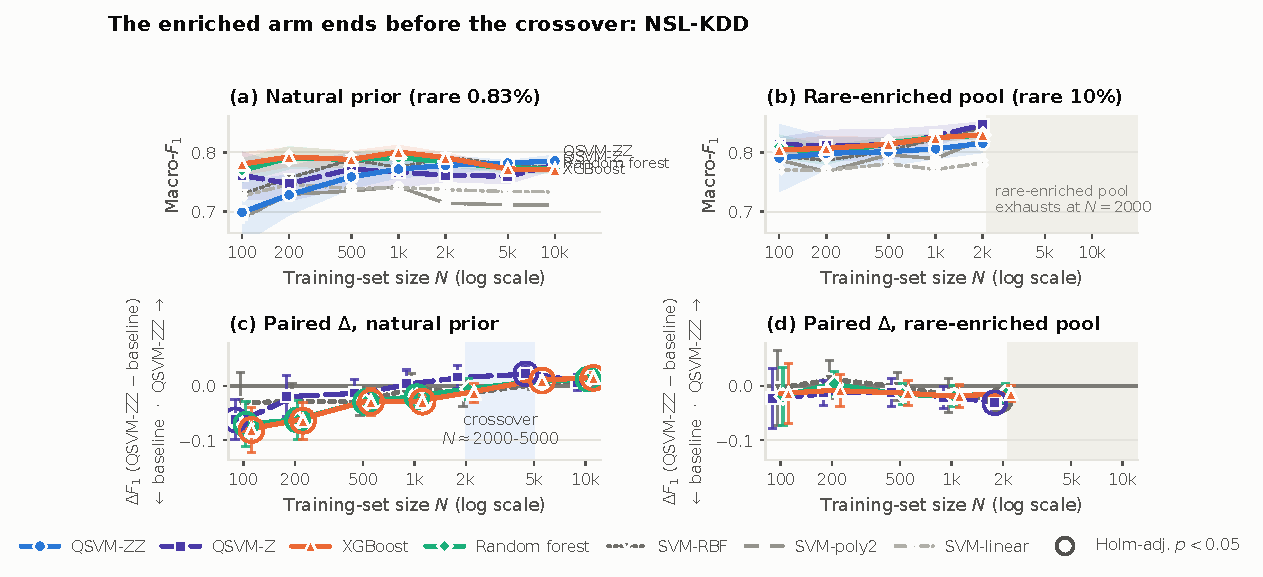
\includegraphics[width=\textwidth]{figs_revision/fig9_learning_curve_nslkdd.pdf}
  \caption{%
    \textbf{Under the natural prior the ordering reverses between $N=2000$ and
    $N=5000$; the rare-enriched arm ends before that interval.} (a,~b) Mean
    macro-$F_1$ over ten runs on the full KDDTest+ set with $95\%$ bands;
    (c,~d) paired differences against each baseline, circled where the
    Holm-adjusted $p<0.05$. The reversal against the tree ensembles and the
    linear and polynomial kernels lies in the band in (c); against SVM-RBF the
    sign change is $+0.0008$ and never significant. The enriched pool (b,~d)
    cannot be sampled past $N=2000$ without runs sharing rare samples, so it
    stops one step before the reversal; within the shared range the tree
    ensembles lead under both priors. Whether enrichment removes the reversal is
    therefore untested, not shown (Sec.~\ref{sec:res-c4}).}
  \label{fig:learning-curve}
\end{figure*}

\input{tables/ref_arm}
\begin{revbody}



The submitted version claimed an advantage in the low-data regime from a sweep
that stopped at $N=1000$. Extending it to $N=10^4$ under the natural class prior
reverses the claim and, in doing so, produces the paper's main new finding
(Fig.~\ref{fig:learning-curve}).

All seven models share the four-component front-end of
Sec.~\ref{sec:framework}, so the ranking below is a ranking of learners on
that embedding. At $N=100$ the ranking is XGBoost $0.7802$, random forest $0.7695$,
QSVM-\Zmap{} $0.7613$, SVM-RBF $0.7296$, linear $0.7261$, \QSVM{} $0.6989$: the
quantum kernel is next to last, and the gap to XGBoost, $-0.0812$, is the
largest in the sweep. At $N=10^4$ the ranking is \QSVM{} $0.7855$, QSVM-\Zmap{}
$0.7787$, SVM-RBF $0.7740$, random forest $0.7728$, XGBoost $0.7706$: the
quantum kernel is first among them. The paired difference against XGBoost passes through
zero between $N=2000$ and $N=5000$ ($-0.0129 \rightarrow +0.0100$), and is
corrected-significant at both $N=5000$ ($p_{\text{Holm}}=0.027$, $d_z=1.22$) and
$N=10^4$ ($+0.0149$, $p_{\text{Holm}}=0.0078$, $d_z=1.07$).

Four qualifications keep this from being read as more than it is.

First, the reversal is not an artefact of re-tuning.
Table~\ref{tab:crossover-arms} repeats the sweep with hyper-parameters frozen at
their C2 values instead of re-tuned at each $N$; all six baseline--arm
combinations change sign in the same interval, $2000\rightarrow5000$. A
re-tuning artefact would not survive freezing the tuning.

Second, the reversal is not uniform across baselines. Against SVM-RBF the
difference does turn positive, but no cell in the sweep reaches
corrected significance; the quantum kernel never demonstrably beats an RBF
kernel at any size we tested. Significance is reached against XGBoost at
$N\geq5000$, against the random forest only at $N=10^4$, and against the linear
and poly-2 kernels from $N=1000$ and $N=2000$ respectively.

Third, whether the reversal is a property of the natural prior cannot be
decided by this design, and an earlier draft of this paper claimed that it was.
Repeating the sweep with rare attacks enriched twelvefold to $10\%$, the
sampling the submitted protocol used, leaves $26$ of $30$ comparisons
inconclusive and shows no crossover in its range; but that range ends at
$N=2000$, because at $N=5000$ the ten runs would share $59\%$ of their rare
samples and independence between runs would be lost, and the crossover under
the natural prior occurs between $N=2000$ and $N=5000$, one step beyond it.
Within the range the two regimes share, the tree ensembles lead under both
priors: against XGBoost the paired difference is negative at all five sizes
under both, against the random forest and SVM-RBF at five of five under the
natural prior and four of five under enrichment, and the sign agrees in $22$ of
the $30$ shared cells; the enriched arm reaches a verdict in $4$ of its $30$
cells against $12$ of $30$ for the natural arm on the same sizes, most of the
difference being classical-favourable cells at $N\leq1000$ that enrichment
leaves inconclusive. The enriched arm therefore ends before the phenomenon begins, and
what the comparison establishes is that enrichment is untested against the
crossover, not that it removes it. What does follow for the submitted protocol
is narrower: a sweep confined to $N\leq2000$, under either prior, could not have
seen the regime in which the kernel does best.

Fourth, the reversal is a statement about the shared embedding, not about the
dataset. Table~\ref{tab:ref-arm} adds a reference arm outside the paired
protocol: XGBoost and the random forest trained on the same nested subsets and
seeds but on all $122$ one-hot features, scored on the same full KDDTest$^+$.
Full-feature XGBoost also declines with $N$ on this split, from
$\refArmXgbPeak$ at $N=\refArmXgbPeakN$ to $\refArmXgbTenK$ at $N=10^4$, and at
$N=5000$ and $N=10^4$ the paired difference against \QSVM{} is
$\refArmDeltaXgbFiveK$ and $\refArmDeltaXgbTenK$: parity, not a crossover.
Against the full-feature random forest the quantum kernel does lead at
$N=10^4$ ($\refArmDeltaRfTenK$). With the entire $125{,}973$-record partition,
full-feature XGBoost reaches $0.804$ (Sec.~\ref{sec:setup}), above the best
score of any four-qubit model in this paper. The practical reading is
therefore narrower than the ranking suggests: a four-qubit kernel matches, but
does not beat, a tree ensemble given the raw record.

\end{revbody}

\subsection{Rare attacks}
\label{sec:res-rare}
\revnote{new}{New subsection. The submitted version claimed ``+6.7 points on rare attacks, d=+0.68'' but the released code computed no rare-class metric (R4-5). That claim is withdrawn.}
\begin{revbody}

Because R2L and U2R are the classes an operator cares about, we report them
separately rather than only inside the macro average. At $N=10^4$ under the
natural prior the rare-class $F_1$ is SVM-RBF $0.585$, \QSVM{} $0.507$,
QSVM-\Zmap{} $0.421$, XGBoost $0.334$, random forest $0.331$, poly-2 $0.109$,
linear $0.089$.

Two things follow. The quantum kernel is far better on rare attacks than either
tree ensemble, which is not visible in the macro average and is worth knowing.
But SVM-RBF is better still, by $0.078$, so the honest statement is that an RBF
kernel is the strongest rare-attack detector in this study. The submitted
version reported a $+6.7$-point rare-attack gain with $d=+0.68$; no rare-class
metric was computed by the code that produced it, and we withdraw the number.
\end{revbody}

\subsection{Transfer to UNSW-NB15}
\label{sec:res-unsw}
\revnote{new}{New subsection. The submitted version mentioned UNSW-NB15 in one sentence of the limitations; AE-3 and R1-2 asked for a second dataset in full.}
\input{figs_revision/fig_unsw_transfer}
\begin{revbody}


The selection rule is applied to UNSW-NB15 without changing a threshold or a
constant (Fig.~\ref{fig:c1-selection}(b)). It returns $n^\ast=6$, at $V=0.9044$,
$\mathrm{KTA}=0.1986$ and $60$ two-qubit gates. Re-running it on ten
independent subsets returns $n^\ast=6$ in $10/10$ at tolerance
$\varepsilon\in\{0.02,0.05\}$ and $7/10$ at $\varepsilon=0.1$. That the rule
returns a different width on a different dataset is the point: it is a rule with
inputs, not a constant dressed as one.

The sample-complexity result does not transfer (Fig.~\ref{fig:unsw-transfer}). At
$N=10^4$, \QSVM{} is favourable against SVM-RBF ($+0.0401$,
$p_{\text{Holm}}=0.0059$) and against its own entanglement-free control
($+0.0449$, $p_{\text{Holm}}=0.0020$), but XGBoost stays ahead at every size
tested ($-0.0204$ at $N=10^4$, classical-favourable), and no crossover against
either tree ensemble occurs anywhere in the sweep. A finding that reproduces on
one dataset and not the other is reported as exactly that.
\end{revbody}

\subsection{Where the kernel breaks, and why}
\label{sec:res-width}
\revnote{new}{New subsection. Answers R3-4 (``very few qubits''): at 8 qubits all 48 comparisons favour the classical side, with the Gram-matrix mechanism measured.}
% Sinh boi runners/make_paper1_figures.py; caption doi chieu bang
% runners/audit_figures.py. File rieng cho tung hinh de \input DUNG CHO
% trong than bai -- float cua LaTeX chi troi VE SAU, khai bao het o cuoi
% tai lieu thi ca 9 hinh don xuong cuoi va tran vao danh muc tai lieu.

\begin{figure*}[t]
  \centering
  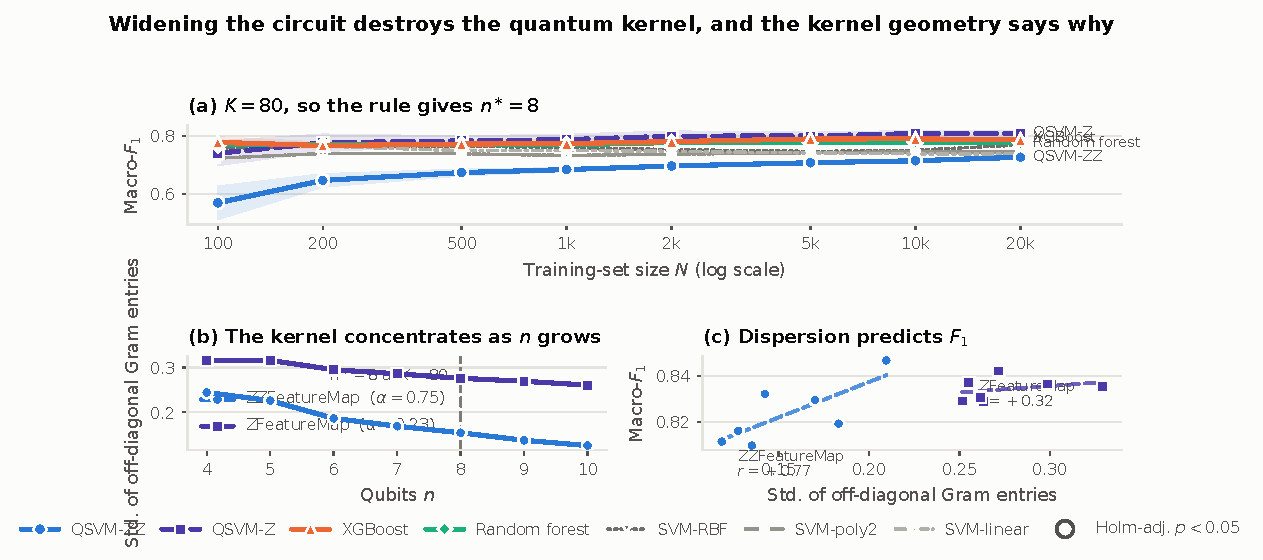
\includegraphics[width=\textwidth]{figs_revision/fig12_width_concentration.pdf}
  \caption{%
    \textbf{Widening the circuit destroys the quantum kernel, and the kernel
    geometry says why.} (a) The sample-complexity sweep re-run at $K=80$, where
    the rule returns $n^{\ast}=8$: all $48$ paired comparisons are
    classical-favourable. (b) Off-diagonal Gram dispersion against width, fitted
    as $n^{-\alpha}$ at $K=80$; the \ZZ{} map concentrates $3.3$ times as fast
    as the \Zmap{} map here ($\alpha=0.75$ against $0.23$), against the factor
    of $2.02$ at $K=20$ that phase-term counting predicts (Sec.~\ref{sec:res-width}).
    (c) Across widths the dispersion correlates with macro-$F_1$ at $r=+0.77$
    for \ZZ{} (95\% CI $[+0.04,+0.96]$) and $r=+0.32$ for \Zmap{}
    ($[-0.57,+0.87]$); the contrast between the two is not resolved at seven
    widths ($z=0.97$, $p=0.33$).}
  \label{fig:width}
\end{figure*}

\begin{revbody}


Sec.~\ref{sec:res-c1} showed that a larger feature budget forces a wider
circuit. Paying that price is the sharpest test of whether the quantum kernel
has headroom, and it fails it (Fig.~\ref{fig:width}).

Re-running the entire sample-complexity sweep at $K=80$, where the rule returns
$n^\ast=8$, produces $48$ paired comparisons (six baselines across eight
training-set sizes), and every one of them is classical-favourable. The
entanglement ablation reverses sign as well: at eight qubits \QSVM{} falls
\emph{below} its entanglement-free control at every size, by $0.082$ to $0.171$
macro-$F_1$. Widening the circuit does not extend the advantage; it removes it.

The mechanism is measurable in the Gram matrix rather than inferred. Writing
$s(n)$ for the standard deviation of the off-diagonal entries and fitting
$s(n)\propto n^{-\alpha}$ over $n=4,\dots,10$, we obtain $\alpha_{\ZZ}=0.590$
against $\alpha_{\Zmap}=0.292$ at $K=20$, a ratio of $2.02$. That ratio is
what the circuit structure predicts: the \ZZ{} map contributes
$\binom{n}{2}$ pairwise phase terms where the \Zmap{} map contributes $n$
single-qubit terms, so the former's phase content grows quadratically and the
latter's linearly. The prediction holds at $K=20$ and not at $K=80$, the budget
at which the collapse occurs: there the fitted exponents are $0.75$ against
$0.23$, a ratio of $3.32$ (Fig.~\ref{fig:width}b), and over the same range the
\ZZ{} kernel loses $49\%$ of its off-diagonal dispersion against $18\%$ for the
\Zmap{} kernel. The counting argument therefore predicts the ordering of the
two decay rates everywhere and their ratio only where the kernel does not
collapse; Sec.~\ref{sec:limitations} returns to this.

The concentration is not merely present; it tracks the end-task result. Across
$n=4,\dots,10$ the correlation between off-diagonal dispersion and macro-$F_1$
is $r=+0.77$ for the \ZZ{} kernel (95\% CI $[+0.04,+0.96]$, $p=0.04$ on seven
widths) and $r=+0.32$ for the \Zmap{} kernel ($[-0.57,+0.87]$, $p=0.48$), which
barely concentrates. The first correlation is resolved, barely; the contrast
between the two is not: a test of the difference between the two correlations
gives $z=0.97$, $p=0.33$, so the data do not establish that the relation is
specific to the concentrating map, and we do not claim that they do. As the Gram
matrix flattens, accuracy follows it down.
This is the exponential-concentration phenomenon of \cite{thanasilp2024} in a
concrete applied setting, and it is why we present a bounded operating window
rather than a method that scales.

An independent measurement supports the boundary and sharpens its
interpretation. Cirillo \emph{et al.} \cite{qmi2026}, sweeping qubit count on
the same corpus under backend-derived noise, locate good performance in a
$20$--$35$ two-qubit-gate band with degradation beyond roughly $60$ gates. Our
operating point of $24$ gates sits inside that band and our collapse at $112$
gates lies beyond their threshold, so the two studies agree on where the
usable window ends. They differ on why: that study attributes the degradation
to two-qubit gate error accumulating on hardware, whereas the results above are
obtained under exact, noiseless simulation, in which no gate error exists. The
window therefore does not widen with better hardware. It is set by the kernel.
\end{revbody}
